\section{Aufgabe 2}
Nach der Justierung der Apparatur wurden die Radien der Ringe nacheinander von uns aufgenommen, welche anschließend mit der Formel
\begin{equation}
r=\frac{1}{2}\cdot (\frac{x_{i,links} + x_{a,links}}{2}-\frac{x_{i,rechts} + x_{a,rechts}}{2}) \notag
\end{equation}
berechnet wurden. Hierbei bezeichnet: \(x_{i/a,links/rechts}\) den Abstand vom Mittelpunkt bis zum inneren/äußeren Rand vom Kreis nach links/rechts. Da  bei der Messung der Radius des ersten Rings nicht bestimmbar war, wird der Radius des zweiten Rings \(r_{z=2}\) als Referenzwert benutzt. Um eine Ursprungsgerade zu erhalten wird der Parameter \(j = z - 2\) eingeführt.
\subsection{Fehlerabschätzung}
Da es sich um eine optische Messung handelt und nur mit der Genauigkeit der Augen gemessen wurde ist von einem großen Fehler auszugehen. Da die erkennbaren Ringe jeweils innen und außen abgemessen wurden, bietet es sich an, deren halbe Dicke als Fehler zu betrachten. Weil es sich um einen Fehler handelt wird die Quadratsumme herangezogen.
\begin{align}
\Delta r &= \frac{1}{2} \cdot \sqrt{
\Delta x_{links}^2 +
\Delta x_{rechts}^2
} \notag \\
&= \frac{1}{2} \cdot \sqrt{
\left( \frac{x_{i,links} - x_{a,links}}{2} \right)^2 +
\left( \frac{x_{i,rechts} - x_{a,rechts}}{2} \right)^2
} \notag
\end{align}
Da nicht \(r\), sondern \( \left( r_0^2 - r_j^2 \right) \) graphisch aufgetragen wird, muss auch dieser Fehler bestimmt werden:
\begin{align}
\Delta \left( r_0^2 - r_j^2 \right) &= \sqrt{
\left( \frac{\partial \left( r_0^2 - r_j^2 \right)}{\partial r_0} \cdot \Delta r_0 \right)^2 +
\left( \frac{\partial \left( r_0^2 - r_j^2 \right)}{\partial r_j} \cdot \Delta r_j \right)^2
} \notag \\
 &= \sqrt{
\left( 2 r_0 \cdot \Delta r_0 \right)^2 +
\left( 2 r_j \cdot \Delta r_j \right)^2
} \notag
\end{align}
\subsection{Gegebenes}
Gegeben ist die Wellenlänge der roten Spektrallinie mit \(\lambda = 643,9\,nm\) und die Brennweite der Objektivlinse mit \(f = (10\pm 0,5)\,cm\). Der Fehler der Wellenlänge ist schwierig abzuschätzen, da er durch Quantenmechanische Unschärfen der Energie entsteht. Es wird im Rahmen dieser  Aufgabe davon ausgegangen, dass er vernachlässigbar klein ist. Zusammengefasst ergibt sich:
\begin{center}
\begin{tabular}{rcc}
\(\lambda\) & \(=\) & \(643,9\, nm\) \\
\(f\) & \(=\) & \(\left( 10,0 \pm 0,5 \right)\, cm\) \\
\end{tabular}
\end{center}
\subsection{Beobachtung}
Im Okular waren, nach guter Positionierung der Objektivlinse, rote Ringe zu sehen. Diese Ringe wurden dann vermessen, indem das im Okular vorhandene Fadenkreuz jeweils auf die Ränder der Ringe ausgerichtet wurde und die Position notiert wurde. Die Position wurde von der Mikrometerschraube abgelesen, mit der auch die Positionierung vorgenommen wurde.
\subsection{Messwerte und Graph}
\begin{center}
\begin{tabular}{c|ccc|ccc|c|c} 
Ordnung \(n\) & \multicolumn{3}{c|}{\(x_{i,links}\)} & \multicolumn{3}{c|}{\(x_{i,rechts}\)} & \(r\) & \(\left( r_i^2 - r_0^2 \right)\)\\
%& i & a & i & a \\
& \multicolumn{3}{c|}{\(mm\)} & \multicolumn{3}{c|}{\(mm\)}  & \(mm\) & \(mm^2\) \\ \hline
\(1\) & N/A & - & \(9,73\) & N/A & - & \(11,78\) & \(1,025\) & \\ 
\(2\) & \(9,48\) & - & \(9,15\) & \(12,01\)  & - & \(12,39\) & \(1,44\pm 0,13\) & \(0,00\pm 0,51\)\\ 
\(3\) & \(8,81\) & - & \(8,52\) & \(12,52\)  & - & \(12,80\) & \(2,00\pm 0,10\) & \(1,91\pm 0,54\)\\ 
\(4\) & \(8,44\) & - & \(8,25\) & \(12,96\)  & - & \(13,22\) & \(2,373\pm 0,081\) & \(3,54\pm 0,53\)\\ 
\(5\) & \(8,08\) & - & \(7,88\) & \(13,36\)  & - & \(13,53\) & \(2,733\pm 0,066\) & \(5,386\pm 0,51\)\\ 
\(6\) & \(7,79\) & - & \(7,60\) & \(13,94\)  & - & \(13,81\) & \(3,020\pm 0,061\) & \(7,04\pm 0,52\)\\ 
\(7\) & \(7,50\) & - & \(7,35\) & \(13,81\)  & - & \(14,08\) & \(3,293\pm 0,052\) & \(8,76\pm 0,50\)\\ 
\(8\) & \(7,24\) & - & \(7,08\) & \(14,17\)  & - & \(14,34\) & \(3,548\pm 0,058\) & \(10,50\pm 0,55\)\\ 
\(9\) & \(7,02\) & - & \(6,90\) & \(14,48\)  & - & \(14,60\) & \(3,790\pm 0,042\) & \(12,28\pm 0,48\)\\ 
\(10\) & \(6,75\) & - & \(6,62\) & \(14,67\)  & - & \(14,77\) & \(4,018\pm 0,041\) & \(14,06\pm 0,49\)\\ 

\end{tabular}
{\it Tab. 2.1: Messwerte für das rote Farbglas (46 803)}
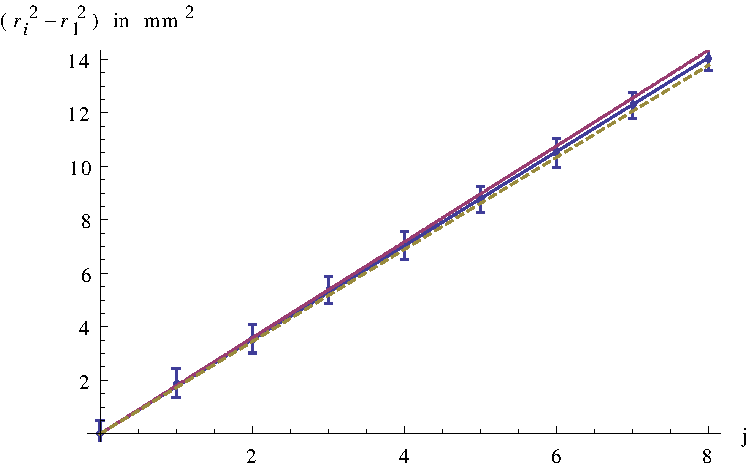
\includegraphics[width=12cm]{rot}
\\
{\it Messwerte mit rotem Glas (46 803) aufgetragen über \(j\)}
\end{center}
Die Steigung \(b\) wurde mittels linearer Regression bestimmt zu
\begin{equation}
b = \left( 1,758 \pm 0,035 \right)\,mm^2
\notag
\end{equation}
\subsection{Auswertung}

Um aus den vorhandenen Messungen auf den Abstand \(d\) der Spiegel zu kommen, wird die Gleichung $\eqref{9}$ herangezogen und \(j = z - 2 \) eingesetzt.
\begin{equation}
j + 2 = \frac{2d}{\lambda}\left(1 - \frac{r_j^2}{2f^2}\right)
\label{j+2}
\end{equation}
Und im Spezialfall \(j=0\)
\begin{align}
2 &= \frac{2d}{\lambda}\left(1 - \frac{r_0^2}{2f^2}\right)
\notag\\
\Rightarrow \frac{2d}{\lambda} &= \frac{2}{1 - \frac{r_0^2}{2f^2}}
\notag
\end{align}
Setzt man das in \eqref{j+2} ein, erhält man:
\begin{align}
j+2 &= 2 \cdot \frac{1 - \frac{r_j^2}{2f^2}}{1 - \frac{r_0^2}{2f^2}} \notag \\
&= 2 \cdot \frac{1 - \frac{r_j^2}{2f^2} - \frac{r_0^2}{2f^2} + \frac{r_0^2}{2f^2}}{1 - \frac{r_0^2}{2f^2}} \notag \\
 &= 2 \cdot \left( \frac{1 - \frac{r_0^2}{2f^2}}{1 - \frac{r_0^2}{2f^2}} + \frac{- \frac{r_j^2}{2f^2} + \frac{r_0^2}{2f^2}}{1 - \frac{r_0^2}{2f^2}}\right) \notag \\
 &= 2 \cdot \left( 1 + \frac{- \frac{r_j^2}{2f^2} + \frac{r_0^2}{2f^2}}{\frac{\lambda}{d}} \right) \notag \\
 &= 2 + \frac{d}{\lambda f^2} \left( r_0^2 - r_j^2 \right) \notag \\
 \Rightarrow j &= \frac{d}{\lambda f^2} \left( r_0^2 - r_j^2 \right) \notag
\end{align}
Somit gilt als Messgleichung: 
\begin{equation}
\left( r_0^2 - r_j^2 \right) = j \cdot \frac{\lambda f^2}{d} \notag
\end{equation}
Mit der Steigung:
\begin{equation}
b = \frac{\lambda f^2}{d}
\label{b}
\end{equation}
Nun ist der Plattenabstand \(d\) bestimmbar durch:
\begin{align}
d &= \frac{\lambda f^2}{b} = 3,66\,mm \notag\\
\Delta d &= d\cdot \sqrt{
\left( \frac{2\Delta f}{f} \right)^2+
\left( \frac{\Delta b}{b} \right)^2
} = 0,16\,mm \notag
\end{align}
\subsection{Fazit}
Da kein Vergleichswert vorliegt, kann der errechnete Plattenabstand nicht verglichen werden. Der vorhandene Fehler wird die Bestimmung der Wellenlänge in Aufgabe 3 ungenau machen. Als Endergebnis für den Plattenabstand wurde
\begin{equation}
d = \left( 3,7 \pm 0,2 \right)\,mm
\notag
\end{equation}
ermittelt.